\section{Knowledge Fragmentation and Duplication? Evidences of Cross-Site Linking}
%\textcolor{blue}{XINGZC: revised introductory paragraph and section 6.2.1. please check.}

ESO and RSO are both programming-related website and our tag usage analysis shows that users of the two sites share much common interests.
Therefore, it is reasonable that some new questions asked in the Russian Stack Overflow may have been already answered or have highly related questions in English Stack Overflow.
This could create knowledge fragmentation and duplication across multi-lingual sites.
But the supporters of multi-lingual sites argue that it is likely that users on non-English Stack Overflow may cross-reference posts to English Stack Overflow, which would solve the knowledge fragmentation and duplication issue.
Below is a user's comment about the concern of knowledge fragmentation and duplication and the suggestion that cross-site linking could solve the issue.	
\begin{comment}
In Q\&A discussions, users often cross-refer existing posts using hyperlinks~\cite{??dehengemseknowledgenetwork}, for example, linking to duplicate questions or related knowledge.
As our tag analysis shows that users of the two sites share some common interests, it is reasonable to expect that some questions in Russian Stack Overflow may have duplicate or related questions in English Stack Overflow.
This could create knowledge fragmentation and duplication across multi-lingual sites.
But the supporters of multi-lingual sites argue that it is likely that users on non-English Stack Overflow may cross-reference posts on English Stack Overflow, which would solve the knowledge fragmentation and duplication issue.
Below is a user's comment about the concern of knowledge fragmentation and duplication and the suggestion that cross-site linking could solve the issue.	
\end{comment}


\begin{comment}
Hyperlink is a good tool to recommend and refer the existing content to other users. 
%Not only links can refer the knowledge base in the same site, but also across different sub-sites, or external resources. 
%Under the site announcement of Japanese Stack Overflow, one user commented, ``''
As Stack Overflow and Russian Stack Overflow are both programming-related website, it is expected that some new questions asked in the Russian Stack Overflow may have already answered or highly related to Stack Overflow.
So there should be some mutual links between them.
In this section, we try to validate such assumptions with the analysis of existing links between them.
%In this section, we explore the relationships between Stack Overflow and Russian Stack Overflow according to their mutual hyperlinks. 
%The link amount and the direction reveal the similarity and difference between these two sites.
\end{comment}

\vspace{2mm}
\noindent \fbox{\centering%
    \parbox{0.98\textwidth}{%
        \textit{``This is the world wide web and it is built on a thing called hypertext. Multiple languages? Cool, that's the "world" part. But don't forget about hypertext. Please, make sure that questions and answers can be linked easily across the different language sites. If someone asks a question in Japanese that is essentially a duplicate of an existing English question, linking the two questions will allow Japanese speakers (who might understand *some* English, or at least be able to read code snippets) to get immediate value from past answers, without waiting for new answers... ''
        }
        
        {\raggedleft --- one comment on the announcement of Japanese Stack Overflow~\cite{web:SOjapanese}\par}
            }%
}
\\

In this section, we investigate existing cross-site links made by the users on Russian Stack Overflow and potential cross-site links that the users are not aware of.
This will provide evidences whether knowledge fragmentation and duplication is a serious issue for multi-lingual sites, whether manual cross-site linking is sufficient to battle this issue, and what kind of tools could better support cross-site linking.

\begin{table}
	\caption{Links statics}
	\centering
	\small
	\label{tab:links}
	\begin{tabular}{llll}
       \hline
		\textbf{Source}      & \textbf{\#Total links} & \textbf{\#Links to ESO}   & \textbf{\#Links to RSO} \\ 
		\hline
		ESO Posts     & 13,636,973    & 1,581,888 (11.6\%)      & 88 \\
		ESO Comments  & 5,959,110     & 1,835,405 (30.8\%)    & 164\\
		RSO Posts    & 131,964       & 5,674  (4.3\%)        & 5,014 (3.8\%) \\
		RSO Comments & 55,471        & 4,548  (8.2\%)        & 5,658 (10.2\%) \\
       \hline
	\end{tabular}

\end{table}	



\subsection{Explicit Cross-Site Links by Users}
\label{sec:explicitLink}
%\textcolor{blue}{ZCXING: not yet revise this section as it is not ready yet.}
%\textcolor{red}{CCY to ZCXING, I know that you are familiar with links in Stack Overflow. Is it suitable for us to categorise links as ``identical'', ``related'', ``un-related''? In addition, someone is saying I tries one link before, but it cannot solve my problem, what kind of link can we count it? Could you please have a look at the part below.}
%\textcolor{blue}{XINGZC: can be four categories: duplicate, related-helpful, related-but-not-helpful, unrelated.}

In Stack Overflow, users can add hyperlinks in their posts (both questions and answers) and comments to reference to other resources. 
We collect all hyperlinks in ESO and RSO and analyse the link direction within and across the two sites.
The statistics of hyperlinks in the two sites are summarised in Table~\ref{tab:links}.
We can see that a large proportion of hyperlinks in ESO posts and comments references to its own content, while only a few hyperlinks in ESO posts and comments reference to the RSO content.
This is unsurprising because English speaking users would not have much interest in Russian content.
In contrast, comparable proportion of hyperlinks in RSO reference to its own content and the ESO content, respectively.
This phenomenon indicates that there could be certain level of knowledge fragmentation and duplication between the two sites and RSO users attempt to address the issue by cross-site linking.

\begin{comment}
The hyperlinks in ESO rarely reference to RSO.
In contrast, many hyperlinks in RSO reference to ESO.
For example, in RSO, 4.3\% hyperlinks in posts and 8.2\% hyperlinks in comments reference to some posts in ESO.
However, compared with RSO, we can see that 11.6\% links in posts and 30.8\% links in comments are from itself in ESO.
%\textcolor{red}{CCY: this argument is a little far-fectched, how to say that more naturally in the paper?}
Such a large difference of link sources leads to two potential reasons: 1) There is not enough overlap content between two sites; 2) ESO may be under-referenced in RSO.
\end{comment}

%In RSO, one question may contain a link to posts (question or answer) in ESO.
%Our task is to see if that assumption holds by checking the retrieval result of our searching model mentioned above.
To further confirm this phenomenon, we manually examine the relationships between a RSO post and an ESO post that is referenced by a hyperlink in the RSO post.
We collect in total 5674 hyperlinks in RSO that reference to ESO.
For each hyperlink, we collect its residing RSO post and the ESO post being referenced.
As we are most familiar with \textit{Python} related questions, we randomly select 50 such pairs of RSO-ESO posts tagged with \textit{Python}.
Examining these 50 pairs of RSO-ESO posts reveal three kinds of relationships between a RSO post and its hyperlinked ESO post: 
duplicate questions (14 pairs), 
related and useful for problem solving (30 pairs), 
and related but not useful for problem solving (6 pairs).

%We assume that such a link represents that the source question in RSO has certain relationship with the target question in ESO.
%According to our observation, there are two kinds of different relationships among these links.
%\textcolor{red}{CCY: Please give detailed number for each category.}

%To systematically define the relationship between each link pair, we categorize the 50 links into three different categories, i.e., identical questions, similar question and not directly relevant questions. 
First, hyperlinks in 14 (28\%) RSO posts reference to some duplicate questions in ESO.
%The identical questions correspond to the refered English Stackoverflow questions which ask the basically same thing as the Russian one. 
For example, the Russian question \foreignlanguage{russian}{"как запустить скрипт на pypy?"}(postid=722948, ``how to run a script on pypy'') has a hyperlink to the English question ``How to use PyPy on Windows?'' (postid=9893317).
Both the Russian question and the English question are about how to run a script of pypy on Windows. 

Second, hyperlinks in 30 (60\%) RSO posts reference to some related but not duplicate English posts in ESO that are useful for solving the problem in the Russian questions.
%In term of the similar question, the pair of the two question ask about the highly relative question under a same topic. 
For example, the Russian question \foreignlanguage{russian}{"Обновление Label из цикла в tkinter"}(postid=581331, ``updating the label of the cycle in tkinter'') has a hyperlink to an ESO post ``Update Tkinter Label from variable'' (postid=2603169). 
The Russian question asks how to use the \textit{update}  function on Tkinter Label in a loop structure.
The referenced ESO question does not solve this specific problem, but it discusses how to use the \textit{update} function, which is relevant. 
%Although they are not duplicate question, they are related and the creator can use that link to help describe their question.
%Tough, the Russian question owner still refered this similar English question to help describe his own question. 
%So we consider this kind of refered questions under a same topic as similar questions.
%But we also find that some reference link are not right or relevant, which are marked as not directly relevant questions.

Third, sometimes RSO users add hyperlinks to the ESO posts in their questions to tell that they have examined some related ESO posts, but these ESO posts cannot solve their problems.
This kind of RSO posts accounts for 6 (12\%) of the 50 examined samples.
%\textcolor{orange}{The original result is just the model output (if model cannot find link pair in top10 result then consider it is related but not helpful), I redo the classification and involved manually checking this time. Data Updated.}
Fo example, one Russian question with the title \foreignlanguage{russian}{"Почему не работает унаследованная форма?"} (postid=318618 `Why does not the inherited form work?'') has a hyperlink to an ESO question ``why does not work in the form of validation?'' (postid=23534615).
The Russian question states that the answers to this ESO question do not work for his problem. 
%After checking these two question, we find that the Russian question wants to find a solution to solve his problem but he mentioned that the method in the referred English question was not working. 

To sum up, the first category of cross-site links reveals knowledge duplication, and the second category may have the risk of knowledge fragmentation.
However, the third category has nothing to do with knowledge fragmentation and duplication.


\begin{comment}
For instance, there is a Russian question, \foreignlanguage{russian}{"Почему нет исключения TypeError?"} (\#564442 "Why is there no TypeError exception?").
Its link in this question leads to the ESO question with title "In Python, how do I determine if an object is iterable?" (\#1952464). 
After manually checking this one pair on the Stack Overflow, we find that he question's owner mentioned one possibility causing the error and \textcolor{red}{refered the link to explain his assumption ???CCY: Do that mean they are related?}. 
So this refered English question is talking about another topic which actually can not deal with this error. So this reference link is not the most suitable one to descripe or solve this russian question.
\end{comment}


%Third, \textcolor{red}{??} links are not right or not suitable in the posts.
%\textcolor{red}{CCY: Give an example about it. }

\begin{comment}
Second, the reference which can not be spotted by our method is due to the limitation of our model. 
Our model focus on capturing and computing the semantic difference between the input words, so currently it may not work well with some deep semantic relationship between words. 
For instance, given an RSO question "\foreignlanguage{russian}{Порядок удаления элементов списка в python}"\footnote{\url{https://ru.stackoverflow.com/questions/55464/}} (translated as "the removal of elements of the list in python"), 
the link inside leads to an English question, "Calling 'del' on a list"\footnote{\url{https://stackoverflow.com/questions/8205102/}}.
In this example, 'del' is obviously a function name for deleting.
However, currently, our model is not able to capture such domain-specific information.
\end{comment}


\subsection{Implicit Cross-site Links that Users Are Not Aware of}
\label{sec:implicitLink}
In Table~\ref{tab:links}, we find that the ratio of hyperlinks in RSO posts and comments that reference to RSO and ESO posts is relatively lower than that of hyperlinks in ESO post and comments that reference to ESO and RSO posts.
This makes us hypothesize that there could be cross-site links between RSO and ESO posts that users are not aware of, and thus have not been explicitly hyperlinked.
%Apart from the existing links mentioned in last subsection, many posts in RSO may also need to add links to ESO, but not done due to the language gap.
To test this hypothesis, we carry out another empirical study. 
As ESO has millions of questions and answers, it is impossible to manually find if a RSO question has some related posts in ESO.
Therefore, we develop a cross-site retrieval method to locate potentially related questions in ESO, given a RSO question.
Then, we analyze the relationships between the given RSO question and the retrieved ESO questions to understand implicit cross-site links.
%Last section analyzes the existing links between two sites, and we are now investigating that if a post 

%But as both Stack Overflow and the Russian one own millions of questions and answers, it is difficult for us to observe to determine which reason accounts for the relative small proportion of links to Stack Overflow.
%Therefore, we propose a cross-site retrieval method to assist our observation and validate the reason mentioned above.

%To understand the scale of implicit cross-site links that the RSO users are not aware of, we develop a cross-site question retrieval method, inspired by~\cite{??bowencrosslingualretrievalemse2017}, to retrieve potentially related questions on English Stack Overflow given a Russian Stack Overflow question.

\begin{figure}
	\centering
	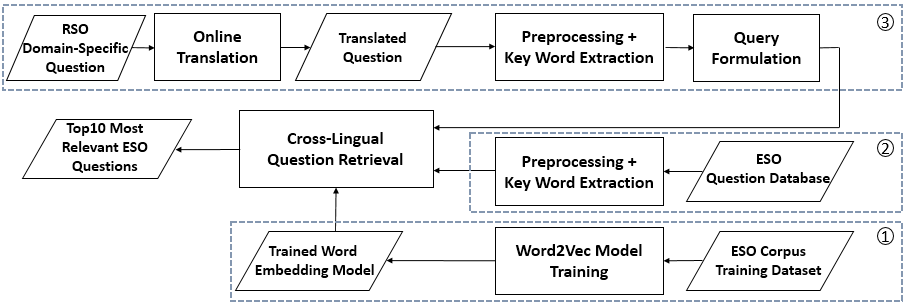
\includegraphics[width = 0.9\textwidth]{figures/workflow.png}
	\caption{Overall framework for cross-site retrieval}
	\centering
	\label{fig:flowChart}
\end{figure}

\begin{figure}
	\centering
	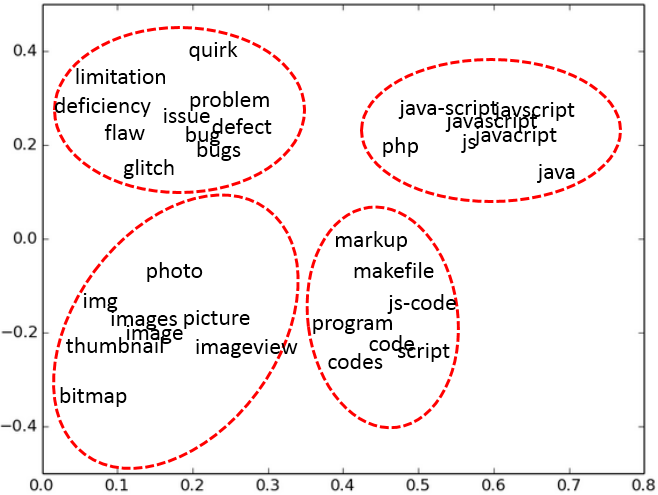
\includegraphics[width = 0.6\textwidth]{figures/PCAplot.png}
	\caption{Visualization of word embeddings by principle component analysis~\cite{jolliffe1986principal}}
	\centering
	\label{fig:PCAimg}
\end{figure}

\subsubsection{Method for cross-site question retrieval}
Fig.~\ref{fig:flowChart} displays the flow chart of our cross-site retrieval method.
The method can be divided into three main parts.
In the first part, we pre-train a word embedding model for retrieving related question for a given query. 
Word embedding~\cite{mikolov2013distributed} is a method to convert the words into dense vectors based on the assumption that words appear in similar context tend to have similar meanings. 
We train a word embedding model using all posts collected from ESO including both question titles and descriptions.
We adopt the Principle Component Analysis~\cite{jolliffe1986principal} to reduce the high-dimensional word embedding into 2-dimension for manual observation.
Examples of some word embeddings are visualized in Fig.~\ref{fig:PCAimg}.
We can see that similar words are close to each other in the vector space, such as ``js'' and ``javascript'', ``image'' and ``picture'', ``bug'' and ``defect''.
In addition, word embedding model is also robust to word morphological transformation (like plural ``images'', ``bugs'') and misspellings (e.g., ``javacript'' and ``jascript'' for ``javascript'').  
Compared with traditional keyword matching, word embedding model helps to bridge the lexical gap between different words which share similar meanings~\cite{chen2016learning}. 

In the second part, we prepare the posts from English Stack Overflow as a question database.
In this study, we build a database of 779,370 ESO questions tagged with \textit{Python}.
We pre-process each question by tokenzing the sentence and removing the stop words in both question title and description.
All words in the question title are considered as keywords.
We extract keywords from the question description because the question description contains too many technical details that could negatively influence the retrieval accuracy. 
We use two different popular keywords extraction algorithms (TF-IDF and TextRank) to extract keywords from the question description. 
TF-IDF (term frequency-inverse document frequency)~\cite{sparck1972statistical} is a numerical metric corresponding to the importance of a word in a corpus.
The TF-IDF metric of a word is proportional to the frequency of the word appearing in one post and inverse proportional to the number of posts in which the word appears.
TextRank~\cite{mihalcea2004textrank} is a popular unsupervised approach for automatic keywords extraction. 
It performs random walk on a graph of word co-occurrences to determine the most important words in a post.
These two algorithms yield two different but complementary sets of keywords. 
To reduce the bias of using a single algorithm, we choose the union of the two keyword sets to build our final set of keywords.
If a keyword appears in both title and description, we consider it as a title keyword.

In the third part, we formulate a RSO question as a query to retrieve related ESO questions in the ESO question database.
We first translate the RSO question's title and description into English with Google Translate~\cite{web:googleTranslate}.
We use the same pre-processing and keyword extraction steps to build a query from the given RSO question.
%We assign different weights to the query keywords from  title and description. 
As question title represents more compact and meaningful information than question description, we assign double weight to title keywords in the query than description keywords.
Given the query of a Russian question ($R$) and an English question ($E$) in the ESO question database, We define the relevance between a query keyword ($R_i$) and a question keyword ($E_j$) as the cosine similarity between the word embeddings of $R_i$ and $E_j$, i.e., $Rel(R_i, E_j)=CosineSim(v_{R_i}, E_j)$. 
For each query keyword $R_i$, we compute its relevance with each keyword of the English Question and find the one with the largest similarity: 
\begin{equation}
Rel(R_i,E)=\max\limits_{j \in E}Rel(R_i, E_j)\times R_i.Weight
\end{equation}
Note that this relevance is weighted by the query keyword's weight $R_i.Weight$.
We then define the relevance between the query of a Russian question ($R$) and an English question ($E$) in the ESO question database as:
\begin{equation}
\label{equ:relevance}
Rel(R, E) = \sum_{i \in R}Rel(R_i, E)
\end{equation}

We compute the relevance of the query and all questions in the ESO question database, and return the top 10 questions with the highest relevance as the most relevant English questions to the given Russian question.

\begin{comment}
%Each question contains two parts, title and descriptions.
\begin{enumerate}
 \item Given one question in Russian Stack overflow, we first translate its title and content description into English with Google Translate\footnote{\url{https://cloud.google.com/translate}}.
 Then we pre-process the translated question by tokenzing the sentence, removing the stop words in both question's title and description.

 \item \textcolor{red}{This step description is wrong! It mixes the two steps in Bowen's approach: 1) build a domain-specific term vocabulary; 2) extract keywords from the question description. I think this need to be separated, otherwise it reads very strange.}
 We extract keywords from the question description because the question description contains too many technical details that could negatively influence the retrieval accuracy. 
 We use two different popular keywords extraction algorithms (TF-IDF and TextRank\footnote{\url{https://github.com/davidadamojr/TextRank}}) to extract keywords from the \textcolor{blue}{ESO question corpus ??should be question description?}. 
 These two algorithms yield two different but complementary sets of keywords. 
 To reduce the bias of using a single algorithm, we choose the union of the two keyword sets to build our final keywords extraction vocabulary.
 Then we only select the keywords which appear in the vocabulary among the query description to improve the retrieval accuracy and speed.
 
 \item We assign different weight to the keywords in title and description. As title represents more compact and meaningful information, we assign double weight to title keywords than description keywords.
 
 \item To build the retrieval model, we adopt the word embedding model. Word embedding~\cite{??} is method to convert the words into dense vectors based on the assumption that words appear in similar context tend to have similar meanings. We trained an word embedding model on posts of Stack Overflow, and some examples can be seen in Fig.~\ref{fig:wordEmbedding}. \textcolor{red}{Add a picture about word2vec + PCA} We can see that similar words \textcolor{red}{....} are relatively close in the vector space. Compared with traditional keyword match, word embedding model can help bridge the lexical gap between different words which share similar meanings. To calculate the relevance between the Russian query ($R$) and an English question ($E$) from the database, we first define the semantic similarity between a query word ($R_i$) and a question word ($E_j$) as the cosine similarity between their learned word embeddings, i.e., $Rel(R_i, E_j)=CosineSim(v_{R_i}, E_j)$. For each query word $R_i$, we compute its similarity with each word in the English Question and find the one with the largest similarity: 
 	 \begin{equation}
       Rel(R_i,E)=\max\limits_{j \in E}Rel(R_i, E_j)\times R_i.Weight
     \end{equation}

     We then define the relevance between a given query \emph{R} and an English question from database \emph{E} as 
      \begin{equation}
      	 \label{equ:relevance}
         Rel(R, E) = \sum_{j\in R}Rel(R_j, E)
      \end{equation}
     We will compare the query with all questions in our database, and sort the relevance value calculated by Equ.\ref{equ:relevance}.
     10 questions with the highest value are extracted as the most relevant questions.
 \end{enumerate}
\end{comment}


\subsubsection{Manual validation of cross-site reference}
%\textcolor{blue}{ZCXING: not yet revise this section as it does not seem ready.}
%There are totally 779,370 questions tagged with \textit{Python} from ESO as the candidate for the query.
%Then we take the question (title and description) in Russian Stack Overflow as the query, and our model returns top-10 related questions in Stack Overflow.
%First, we use the 50 RSO questions in Section~\ref{sec:explicitLink} as query questions and obtain the top-10 related ESO question using our cross-site retrieval method.
We randomly sampled 50 RSO questions tagged with \textit{Python} that do not have hyperlinks to ESO. 
We use these RSO questions as query questions and obtain the top-10 related ESO questions for each RSO question using our cross-site retrieval method.
We then examine if the retrieved ESO questions are duplicate or otherwise related to the query RSO questions.  
%We regard them as the queries, and to see if we can find any identical or related questions in Stack Overflow in the top-10 retrieval results.
 
We find that for 6 (12\%) RSO questions, we can locate duplicate questions in the top-10 ESO questions returned by our cross-site retrieval method. 
For the other 20 (40\%) Russian questions, we can locate at least one related-but-not-duplicate ESO questions in the top-10 list. 
Table~\ref{tab:reviewresult} presents three RSO questions (title translated into English) in our study.
We only show the top 3 most relevant ESO questions due to the space limit. 
Among these three examples, our cross-site retrieval method finds a duplicate ESO question (postid=9694065,  ``Searching for a Python lightweight IDE (or text-editor)'') to the RSO question (postid=464, ``IDE for Python'') and finds some related ESO questions to the RSO questions (postid=432934, ``The slow implementation of the code a coin toss, and postid=420125, ``Books and educational resources for Python'').

For the rest 24 (48\%) RSO questions, Our cross-site retrieval method does not find any related questions in the current ESO database.
Note that it may be either due to the limitation of our method, or the fact that there are no duplicate or related questions in ESO. 
More future works are needed to confirm the detailed reasons.

 \begin{table}
 \caption{Examples from implicit cross-site links that users are not aware of}
 \centering
 \tiny
 \label{tab:reviewresult}
 \begin{tabular}{|p{0.8cm}|p{3.9cm}|p{3.9cm}|p{3.9cm}|}
 	%\hline
	%Russian Question &{\emph \foreignlanguage{russian}{IDE для Python}} & {\emph \foreignlanguage{russian}Отладка кода на Питоне}} &{\emph \foreignlanguage{russian} {Python обработчик системного меню Windows}\\ 
 	\hline
 	Translated Question & IDE for python (\#464) & the slow implement of the code, a coin toss (\#432934) & books and educational resources for python (\#420125)\\
 	\hline
 	Result \#1 & [duplicated] Searching for a Python lightweight IDE (or text-editor) (\#6011678) &  [related] python code for coin toss issues (\#6486877) & [related] Resource/book suggestion to effectively writing software for python/c++ beginner (\#9694065)\\
 	\hline
 	Result \#2 & [related] What's a good IDE for Python on Mac OS X? (\#893162) & [related] python coin toss (\#14882530) & [related] good resource for learning advanced or obscure python concepts (\#14756145) \\
 	\hline
 	Result \#3 & [related] IDE for Python: test a script (\#6023377) & [related] Simulate multipe coin toss streak (\#15761259) & [related] what are good online resources to learn using Pyhton to get and post data in a webpage? (\#41241481)\\
	
 	\hline
 \end{tabular}
 
 \end{table}

\vspace{2mm}
\noindent \fbox{\centering%
	\parbox{0.98\textwidth}{%

      \textbf{Summary}: 
      There are certain level of knowledge fragmentation and duplication across ESO and RSO.
      RSO users recognize some duplicate and related ESO posts and reference them in RSO posts and comments.
      But there are many duplicate and related ESO questions that RSO users are not aware of and thus do not reference in RSO posts, which calls for tool support to better tackle knowledge fragmentation and duplication issue.
       %Many hyperlinks in Russian Stack Overflow come from the main site which shows the Stack Overflow is an important information resource for the Russian one.
       %But there are still two problems with it, one is that some existing links are not related or not most related.
       %Second, some reference links are missing and need the support of some tools.
  }
}